\documentclass[12pt,letterpaper]{hmcpset}
\usepackage[margin=1in]{geometry}
\usepackage{graphicx}
\usepackage{amsthm}
\usepackage{enumitem}

% Theorems
\usepackage{amsthm}
\renewcommand\qedsymbol{$\blacksquare$}
\makeatletter
\@ifclassloaded{article}{
    \newtheorem{definition}{Definition}[section]
    \newtheorem{example}{Example}[section]
    \newtheorem{theorem}{Theorem}[section]
    \newtheorem{corollary}{Corollary}[theorem]
    \newtheorem{lemma}{Lemma}[theorem]
}{
}
\makeatother

% Random Stuff
\setlength\unitlength{1mm}

\newcommand{\insertfig}[3]{
\begin{figure}[htbp]\begin{center}\begin{picture}(120,90)
\put(0,-5){\includegraphics[width=12cm,height=9cm,clip=]{#1.eps}}\end{picture}\end{center}
\caption{#2}\label{#3}\end{figure}}

\newcommand{\insertxfig}[4]{
\begin{figure}[htbp]
\begin{center}
\leavevmode \centerline{\resizebox{#4\textwidth}{!}{\input
#1.pstex_t}}
\caption{#2} \label{#3}
\end{center}
\end{figure}}

\long\def\comment#1{}

\newcommand\norm[1]{\left\lVert#1\right\rVert}
\DeclareMathOperator*{\argmin}{arg\,min}
\DeclareMathOperator*{\argmax}{arg\,max}

% bb font symbols
\newfont{\bbb}{msbm10 scaled 700}
\newcommand{\CCC}{\mbox{\bbb C}}

\newfont{\bbf}{msbm10 scaled 1100}
\newcommand{\CC}{\mbox{\bbf C}}
\newcommand{\PP}{\mbox{\bbf P}}
\newcommand{\RR}{\mbox{\bbf R}}
\newcommand{\QQ}{\mbox{\bbf Q}}
\newcommand{\ZZ}{\mbox{\bbf Z}}
\renewcommand{\SS}{\mbox{\bbf S}}
\newcommand{\FF}{\mbox{\bbf F}}
\newcommand{\GG}{\mbox{\bbf G}}
\newcommand{\EE}{\mbox{\bbf E}}
\newcommand{\NN}{\mbox{\bbf N}}
\newcommand{\KK}{\mbox{\bbf K}}
\newcommand{\KL}{\mbox{\bbf KL}}

% Vectors
\renewcommand{\aa}{{\bf a}}
\newcommand{\bb}{{\bf b}}
\newcommand{\cc}{{\bf c}}
\newcommand{\dd}{{\bf d}}
\newcommand{\ee}{{\bf e}}
\newcommand{\ff}{{\bf f}}
\renewcommand{\gg}{{\bf g}}
\newcommand{\hh}{{\bf h}}
\newcommand{\ii}{{\bf i}}
\newcommand{\jj}{{\bf j}}
\newcommand{\kk}{{\bf k}}
\renewcommand{\ll}{{\bf l}}
\newcommand{\mm}{{\bf m}}
\newcommand{\nn}{{\bf n}}
\newcommand{\oo}{{\bf o}}
\newcommand{\pp}{{\bf p}}
\newcommand{\qq}{{\bf q}}
\newcommand{\rr}{{\bf r}}
\renewcommand{\ss}{{\bf s}}
\renewcommand{\tt}{{\bf t}}
\newcommand{\uu}{{\bf u}}
\newcommand{\ww}{{\bf w}}
\newcommand{\vv}{{\bf v}}
\newcommand{\xx}{{\bf x}}
\newcommand{\yy}{{\bf y}}
\newcommand{\zz}{{\bf z}}
\newcommand{\0}{{\bf 0}}
\newcommand{\1}{{\bf 1}}

% Matrices
\newcommand{\Ab}{{\bf A}}
\newcommand{\Bb}{{\bf B}}
\newcommand{\Cb}{{\bf C}}
\newcommand{\Db}{{\bf D}}
\newcommand{\Eb}{{\bf E}}
\newcommand{\Fb}{{\bf F}}
\newcommand{\Gb}{{\bf G}}
\newcommand{\Hb}{{\bf H}}
\newcommand{\Ib}{{\bf I}}
\newcommand{\Jb}{{\bf J}}
\newcommand{\Kb}{{\bf K}}
\newcommand{\Lb}{{\bf L}}
\newcommand{\Mb}{{\bf M}}
\newcommand{\Nb}{{\bf N}}
\newcommand{\Ob}{{\bf O}}
\newcommand{\Pb}{{\bf P}}
\newcommand{\Qb}{{\bf Q}}
\newcommand{\Rb}{{\bf R}}
\newcommand{\Sb}{{\bf S}}
\newcommand{\Tb}{{\bf T}}
\newcommand{\Ub}{{\bf U}}
\newcommand{\Wb}{{\bf W}}
\newcommand{\Vb}{{\bf V}}
\newcommand{\Xb}{{\bf X}}
\newcommand{\Yb}{{\bf Y}}
\newcommand{\Zb}{{\bf Z}}

% Calligraphic
\newcommand{\Ac}{{\cal A}}
\newcommand{\Bc}{{\cal B}}
\newcommand{\Cc}{{\cal C}}
\newcommand{\Dc}{{\cal D}}
\newcommand{\Ec}{{\cal E}}
\newcommand{\Fc}{{\cal F}}
\newcommand{\Gc}{{\cal G}}
\newcommand{\Hc}{{\cal H}}
\newcommand{\Ic}{{\cal I}}
\newcommand{\Jc}{{\cal J}}
\newcommand{\Kc}{{\cal K}}
\newcommand{\Lc}{{\cal L}}
\newcommand{\Mc}{{\cal M}}
\newcommand{\Nc}{{\cal N}}
\newcommand{\Oc}{{\cal O}}
\newcommand{\Pc}{{\cal P}}
\newcommand{\Qc}{{\cal Q}}
\newcommand{\Rc}{{\cal R}}
\newcommand{\Sc}{{\cal S}}
\newcommand{\Tc}{{\cal T}}
\newcommand{\Uc}{{\cal U}}
\newcommand{\Wc}{{\cal W}}
\newcommand{\Vc}{{\cal V}}
\newcommand{\Xc}{{\cal X}}
\newcommand{\Yc}{{\cal Y}}
\newcommand{\Zc}{{\cal Z}}

% Bold greek letters
\newcommand{\alphab}{\hbox{\boldmath$\alpha$}}
\newcommand{\betab}{\hbox{\boldmath$\beta$}}
\newcommand{\gammab}{\hbox{\boldmath$\gamma$}}
\newcommand{\deltab}{\hbox{\boldmath$\delta$}}
\newcommand{\etab}{\hbox{\boldmath$\eta$}}
\newcommand{\lambdab}{\hbox{\boldmath$\lambda$}}
\newcommand{\epsilonb}{\hbox{\boldmath$\epsilon$}}
\newcommand{\nub}{\hbox{\boldmath$\nu$}}
\newcommand{\mub}{\hbox{\boldmath$\mu$}}
\newcommand{\zetab}{\hbox{\boldmath$\zeta$}}
\newcommand{\phib}{\hbox{\boldmath$\phi$}}
\newcommand{\psib}{\hbox{\boldmath$\psi$}}
\newcommand{\thetab}{\hbox{\boldmath$\theta$}}
\newcommand{\taub}{\hbox{\boldmath$\tau$}}
\newcommand{\omegab}{\hbox{\boldmath$\omega$}}
\newcommand{\xib}{\hbox{\boldmath$\xi$}}
\newcommand{\sigmab}{\hbox{\boldmath$\sigma$}}
\newcommand{\pib}{\hbox{\boldmath$\pi$}}
\newcommand{\rhob}{\hbox{\boldmath$\rho$}}

\newcommand{\Gammab}{\hbox{\boldmath$\Gamma$}}
\newcommand{\Lambdab}{\hbox{\boldmath$\Lambda$}}
\newcommand{\Deltab}{\hbox{\boldmath$\Delta$}}
\newcommand{\Sigmab}{\hbox{\boldmath$\Sigma$}}
\newcommand{\Phib}{\hbox{\boldmath$\Phi$}}
\newcommand{\Pib}{\hbox{\boldmath$\Pi$}}
\newcommand{\Psib}{\hbox{\boldmath$\Psi$}}
\newcommand{\Thetab}{\hbox{\boldmath$\Theta$}}
\newcommand{\Omegab}{\hbox{\boldmath$\Omega$}}
\newcommand{\Xib}{\hbox{\boldmath$\Xi$}}

% mixed symbols
\newcommand{\sinc}{{\hbox{sinc}}}
\newcommand{\diag}{{\hbox{diag}}}
\renewcommand{\det}{{\hbox{det}}}
\newcommand{\trace}{{\hbox{tr}}}
\newcommand{\tr}{\trace}
\newcommand{\sign}{{\hbox{sign}}}
\renewcommand{\arg}{{\hbox{arg}}}
\newcommand{\var}{{\hbox{var}}}
\newcommand{\cov}{{\hbox{cov}}}
\renewcommand{\Re}{{\rm Re}}
\renewcommand{\Im}{{\rm Im}}
\newcommand{\eqdef}{\stackrel{\Delta}{=}}
\newcommand{\defines}{{\,\,\stackrel{\scriptscriptstyle \bigtriangleup}{=}\,\,}}
\newcommand{\<}{\left\langle}
\renewcommand{\>}{\right\rangle}
\newcommand{\Psf}{{\sf P}}
\newcommand{\T}{\top}
\newcommand{\m}[1]{\begin{bmatrix} #1 \end{bmatrix}}


% info for header block in upper right hand corner
\name{}
\class{Math189R SP19}
\assignment{Homework 1}
\duedate{Monday, Feb 4, 2017}

\renewcommand{\labelenumi}{{(\alph{enumi})}}


\begin{document}
Feel free to work with other students, but make sure you write up the homework
and code on your own (no copying homework \textit{or} code; no pair programming).
Feel free to ask students or instructors for help debugging code or whatever else,
though.
The starter code for problem 2 part c and d can be found under the Resource tab on course website.\\

\textit{Note:} You need to create a Github account for submission of the coding part of the homework. Please create a repository on Github to hold all your code and include your Github account username as part of the answer to problem 2.

\begin{problem}[1]
(\textbf{Linear Transformation}) Let $\mathbf{y} = A\mathbf{x} + \mathbf{b}$ be a random vector.
show that expectation is linear:
\[
    \EE[\yy] = \EE[A\xx + \bb] = A\EE[\xx] + \bb.
\]
Also show that
\[
    \cov[\yy] = \cov[A\xx + \bb] = A \cov[\xx] A^\T = A\Sigmab A^\T.
\]
\end{problem}
\begin{solution} 

	We wish to show that \EE[\yy] = \EE[A\xx + \bb] = A\EE[\xx] + \bb. By definition of expectation, we have $$\EE[\yy] = \int_S(A\xx + \bb)\PP(x)dx,$$ where $S$ is the space contains all possible $x$. Then, we can rearrange to get $$\EE[\yy] =  A\int_S\xx \PP(x)dx +  \bb\int_S\PP(x)dx.$$ Note that by definition of expectation, $\EE[\xx] =\int_S\xx \PP(x)dx$. Also by definition of random variables $\int_S\PP(x)dx =1$. Thus, we can see that $\EE[\yy] =  A\EE[\xx] +  \bb.$\\
    	
    Next, we wish to show that $\cov[\yy] = \cov[A\xx + \bb] = A \cov[\xx] A^\T = A\Sigmab A^\T.$ We are given $\yy = A\xx + \bb$ so that $\cov[\yy] = \cov[A\xx+\bb]$. Then, by definition of covariance, we have $\cov[A\xx+\bb] = \EE[(A\xx+b - \EE[A\xx+b])(A\xx+b - \EE[A\xx+b])^T]$. By linearity of expectation, we can rewrite as $\cov[A\xx+\bb] = \EE[(A\xx+b - A\EE[\xx] - b)(A\xx+b - A\EE[\xx]-b)^T]$. Simplifying, we get $\cov[A\xx+\bb] = \EE[(A\xx - A\EE[\xx])(A(\xx- \EE[\xx]))^T]$. Applying transpose in the second term inside expectation, we get $\cov[A\xx+\bb] = \EE[(A\xx - A\EE[\xx])(\xx- \EE[\xx])^TA^T]$. Since $A$ and $A^T$ are constants, by linearity, we have $\cov[A\xx+\bb] = A\EE[(\xx - A\EE[\xx])(\xx- \EE[\xx])^T]A^T$. Lastly, by definition of covariance, we see $\cov[A\xx+\bb] = A\cov[\xx]A^T = A\Sigmab A^T$ as desired.
\end{solution}
\newpage


\begin{problem}[2]
Given the dataset $\Dc = \{(x,y)\} = \{(0,1), (2,3), (3,6), (4,8)\}$
\begin{enumerate}
   \item Find the least squares estimate $y = \thetab^\T\xx$ by hand using
        Cramer's Rule.
    \item Use the normal equations to find the same solution and verify it
        is the same as part (a).
    \item Plot the data and the optimal linear fit you found.
    \item Find randomly generate 100 points near the line with white Gaussian
        noise and then compute the least squares estimate (using a computer).
        Verify that this new line is close to the original and plot the new
        dataset, the old line, and the new line.
\end{enumerate}

\end{problem}
\begin{solution}
    \begin{enumerate}
    	\item Let $$X = \begin{bmatrix}
1 & 0 \\
1 & 2 \\
1 & 3 \\
1 & 4
\end{bmatrix}\text{ and } \yy = \begin{bmatrix}
1 \\
3 \\
6 \\
8
\end{bmatrix}.$$
To find the least square estimate using Cramer's Rule, we need to set $X^TX \theta = X^T\yy$ where $\theta = \begin{bmatrix}
	\theta_0\\
	\theta_1
\end{bmatrix}$. Plugging in, we get $$X^TX\theta = \begin{bmatrix}
	4 & 9\\
	9 & 29
\end{bmatrix}\begin{bmatrix}
	\theta_0\\
	\theta_1
\end{bmatrix} = X^T\yy = \begin{bmatrix}
	18\\
	56
\end{bmatrix}.$$
Next, we apply Cramer's Rule to solve for $\theta_0$ and $\theta_1$. $$\theta_0 =\frac{
\begin{vmatrix}
18 & 9 \\
56 & 29
\end{vmatrix}
}{
\begin{vmatrix}
4 & 9 \\
9 & 29
\end{vmatrix}
} = \frac{18}{35} \text{ and }\theta_1 =\frac{
\begin{vmatrix}
4 & 18 \\
9 & 56
\end{vmatrix}
}{
\begin{vmatrix}4 & 9 \\
9 & 29
\end{vmatrix}
} = \frac{62}{35}$$

Thus, for the given dataset,  we found the least square estimate is $y = \frac{18}{35} +\frac{62}{35}x$ using Cramer's Rule

\newpage
\item Using the normal equation we can solve for $\theta$ using the following formula,
$$\theta = (X^TX)^{-1}X^T\yy.$$ Then, we can plug in values from part a and evaluate, $$\theta = \begin{bmatrix}
	4 & 9\\
	9 & 29
\end{bmatrix}^{-1} \begin{bmatrix}
	1 & 1 & 1 & 1\\
	0 & 2 & 3 & 4
\end{bmatrix}\begin{bmatrix}
1 \\
3 \\
6 \\
8
\end{bmatrix} = \begin{bmatrix}
\frac{18}{35}\\
\frac{62}{35}
\end{bmatrix}.$$
Thus, we see that the solution using the normal equation is the same as using Cramer's rule as in part a.

\item Plotted data and optimal linear fit.

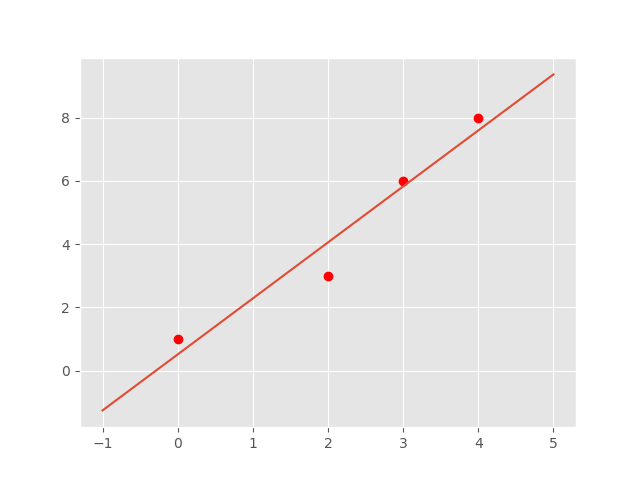
\includegraphics{hw1pr2c.png}
\newpage
\item Plotted data with Gaussian noise and new least square estimate. Note that the new line is close to the old line.

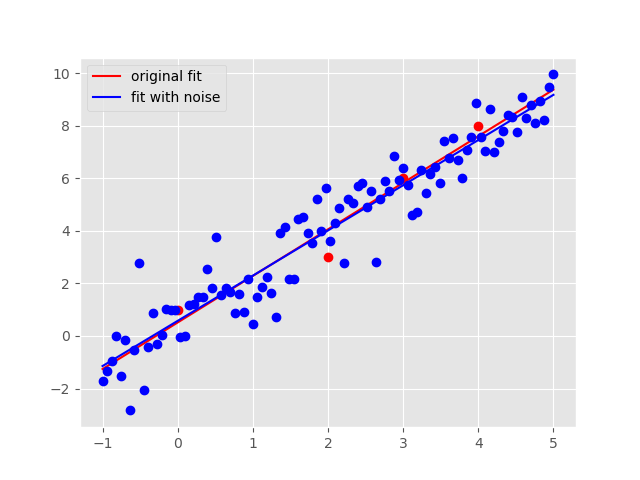
\includegraphics{hw1pr2d.png}
    \end{enumerate}


\end{solution}
\newpage



\end{document}